\documentclass[aspectratio=169,11pt,hyperref={colorlinks=true}]{beamer}
\usepackage[utf8]{inputenc}
\usepackage[T1]{fontenc}
\usepackage{fontspec}
\usepackage[absolute,overlay]{textpos}
\usepackage{listingsutf8}
\usepackage{listings-golang}
\usepackage{tikz}
\usepackage{color}
\usepackage{fontawesome5}
\usepackage{svg}


\title{Adopting CDEvents and Embracing Interoperability}
\date[16 April 2024]{cdCon @ OSSNA | 16 April 2024 | \faTwitter ~@\_cdevents | \faGithub ~cdevents}
\author[Andrea Frittoli]{%
  Andrea Frittoli \\
  Developer Advocate @ IBM\\
  andrea.frittoli@uk.ibm.com \\
  \faTwitter ~@blackchip76 | \faGithub ~afrittoli\\
  ~\\
  Session: \href{https://sched.co/1aBN2}{sched.co/1aBN2}
}

\usetheme{af}

% Code style
\setlststyle

\lstdefinelanguage{koyaml}{
  keywords={github, com, afrittoli, examples, ms, go, helloworld},
  sensitive=false,
  comment=[l]{\#},
  morestring=[b]',
  morestring=[b]"
}

% Automatic section frame
% \AtBeginSection{\frame{\sectionpage}}

\begin{document}

\begin{frame}
\titlepage{}
\end{frame}

\begin{speakerframe}[af_wind.jpg]{Andrea Frittoli}%
  {%
  \faGithub ~afrittoli | \faLinkedin ~andreafrittoli | \faTwitter ~@blackchip76
  }%
  {%
  \begin{itemize}
    \item{Open Source Advocate @ IBM}
    \item{Lives in Wales, enjoys the wind}
    \item{CDEvents maintainer, Events SIG co-chair}
    \item{Chair of CDF Technical Oversight Committee \\ Governing Board}
  \end{itemize}
  }%
\end{speakerframe}

\begin{lpicrblack}[calum-lewis-vA1L1jRTM70-unsplash.jpg]{%
  Photo by \href{https://unsplash.com/@calumlewis}{\underline{Calum Lewis}}, CC0
  }%
  {%
  \tableofcontents
  }%
  {}
  \frametitle{~~~~~~~~~~~~~~~~~~~~~~~~~~~~~~~~~~~~~~~~~~~~~~~~~~~Contents}
\end{lpicrblack}

\section[Software Factory]{Software Factory}

\begin{sectionwithpiclargecentral}[jezael-melgoza-HYQvV8wWX18-unsplash.jpg]{Photo by \href{https://unsplash.com/@jezar}{\underline{Jezael Melgoza}}, CC0}
\end{sectionwithpiclargecentral}
\note[itemize]{
  \item Use some factory picture
}

\begin{grayframe}
  \frametitle{Software Factory}
  \begin{textblock*}{0.70\paperwidth}(0.15\paperwidth,0.20\paperheight)
    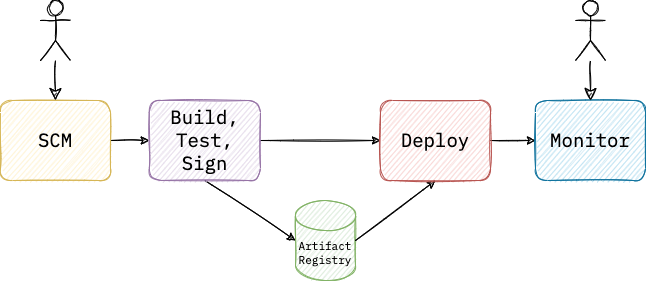
\includegraphics[width=0.70\paperwidth]{img/cdevents-1-no-events.png}
  \end{textblock*}
\end{grayframe}
\note[itemize]{
  \item Problem statement part 1 - Glue Code, Lack of Scalability
  \item A couple of slides
  \item 1. Simple build system
  \item 2. Multiple components, more requirements (glue code)
  \item Use existing diagrams, the second diagram from the google slides version
}

\begin{blackframe}
  \frametitle{Software Factory}
  \begin{itemize}
    \item "Glue code" explosion
    \item Does not scale
    \item Expensive to onboard \\new services
    \item Hard to maintain
  \end{itemize}
  \begin{textblock*}{0.60\paperwidth}(0.35\paperwidth,0.13\paperheight)
    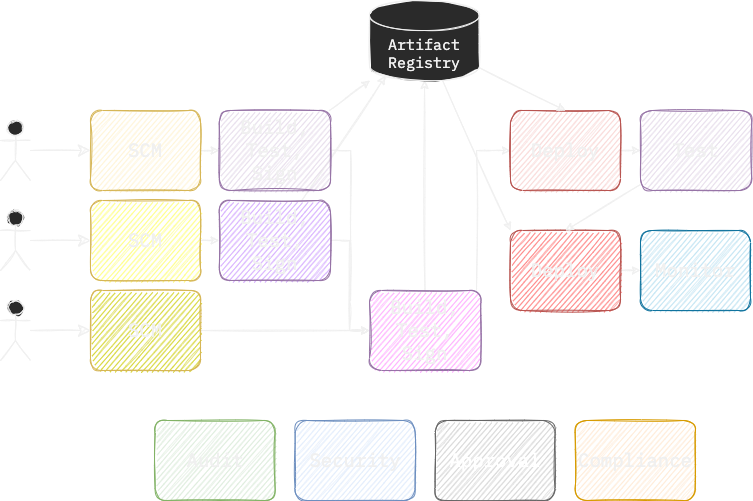
\includegraphics[width=0.60\paperwidth]{img/cdevents-multiple-components.png}
  \end{textblock*}
\end{blackframe}
\note[itemize]{
  \item 2. Multiple components, more requirements (glue code)
  \item Use existing diagrams, the second diagram from the google slides version
}

\begin{grayframe}
  \frametitle{Internal Development Platform}
  \begin{textblock*}{0.70\paperwidth}(0.15\paperwidth,0.20\paperheight)
    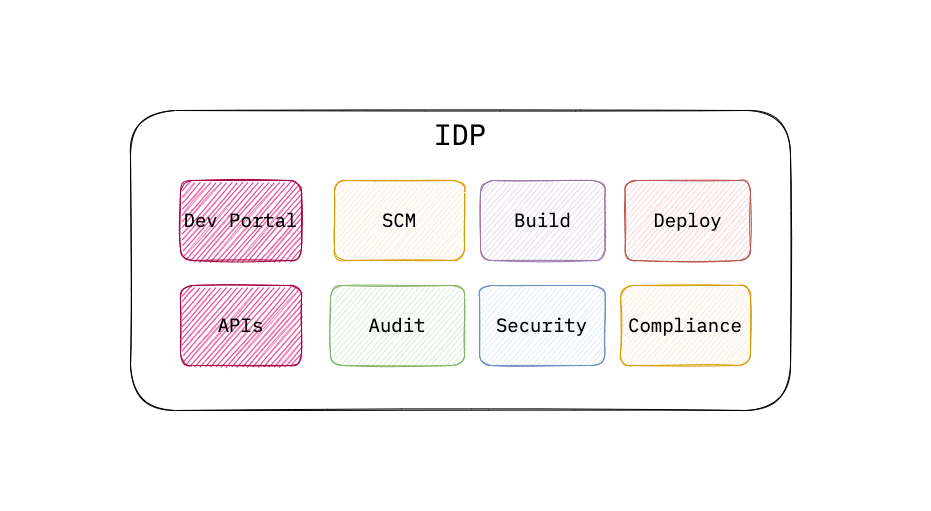
\includegraphics[width=0.70\paperwidth]{img/cdevents-idp.png}
  \end{textblock*}
\end{grayframe}
\note[itemize]{
  \item Problem statement part 2 - Lock in effect, Loss of data
  \item A couple of slides
  \item 1. IDP architecture
  \item 2. Multiple triggers, 1 dashboard, evidence store (metrics, audit)
  \item Draw two diagrams with IDP
}

\begin{blackframe}
  \frametitle{Internal Development Platform}
  \begin{itemize}
    \item Lock-in effect
    \item Missing/Broken Data
    \item Many Dashboards
  \end{itemize}
  \begin{textblock*}{0.60\paperwidth}(0.35\paperwidth,0.13\paperheight)
    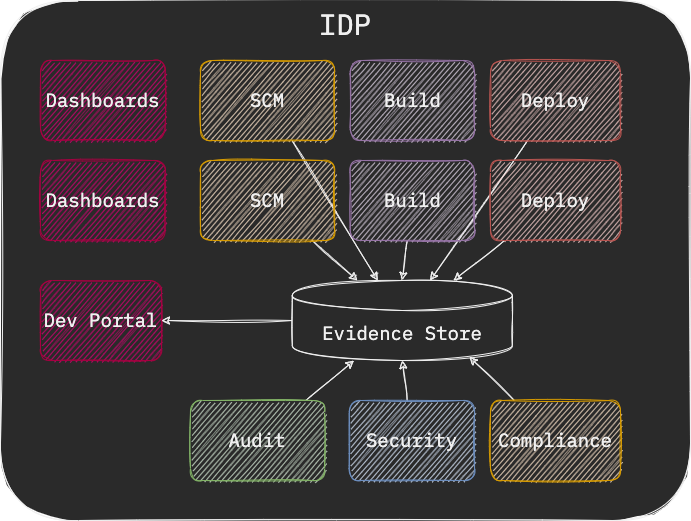
\includegraphics[width=0.60\paperwidth]{img/cdevents-idp-multiple.png}
  \end{textblock*}
\end{blackframe}
\note[itemize]{
  \item 2. Multiple triggers, 1 dashboard, evidence store (metrics, audit)
  \item Draw two diagrams with IDP
}

\begin{grayframe}
  \frametitle{A Plethora of Tools}
  \begin{textblock*}{1.0\paperwidth}(0\paperwidth,0.18\paperheight)
    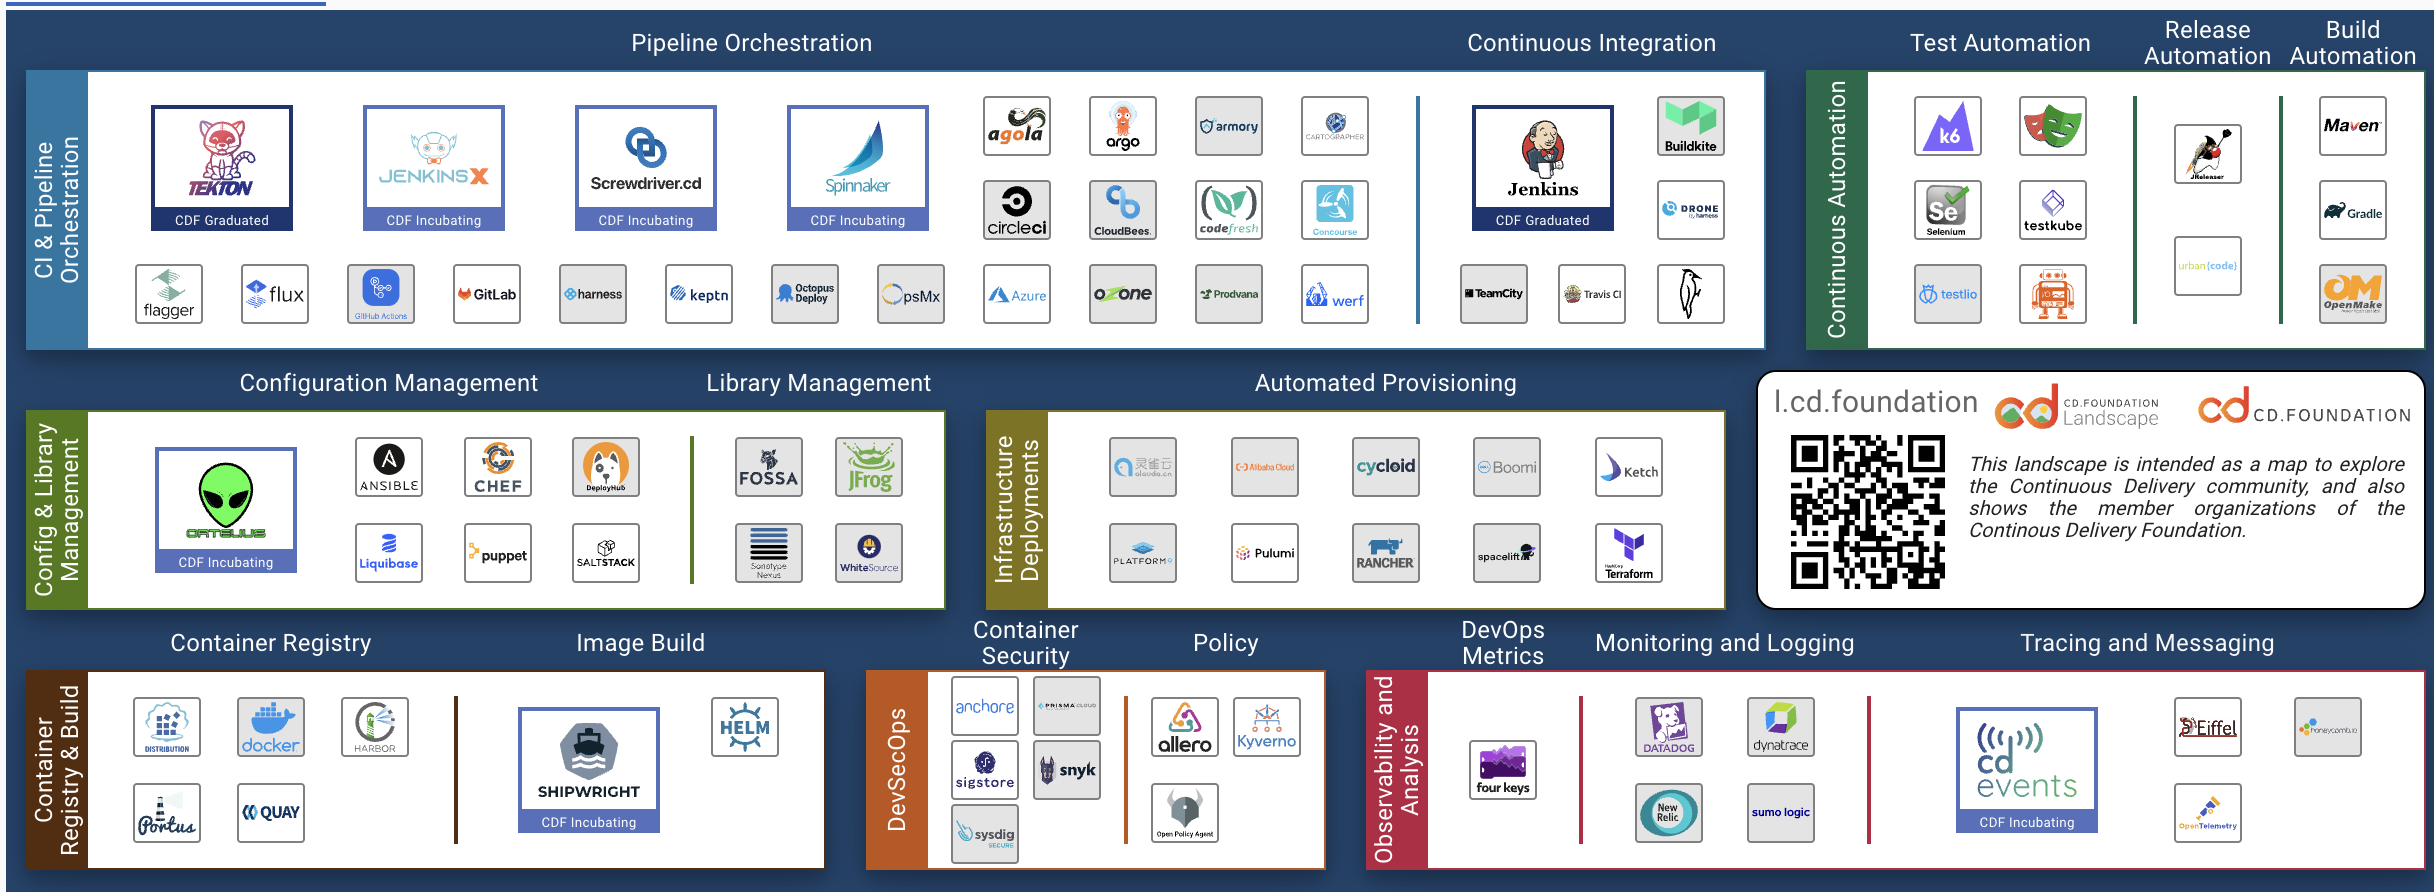
\includegraphics[width=1.0\paperwidth]{img/landscape.cd.foundation.png}
  \end{textblock*}
\end{grayframe}
\note[itemize]{
  \item We need multiple tools to satisfy requirements, improve metrics
  \item Added complexity, risk, skills required
  \item We need data to satisfy requirements
  \item Mention slashdata report
  \item Use the landscape diagram
}

\begin{blackframe}
  \frametitle{State of CI/CD Report 2024}
  \begin{textblock*}{0.4\paperwidth}(0.07\paperwidth,0.18\paperheight)
    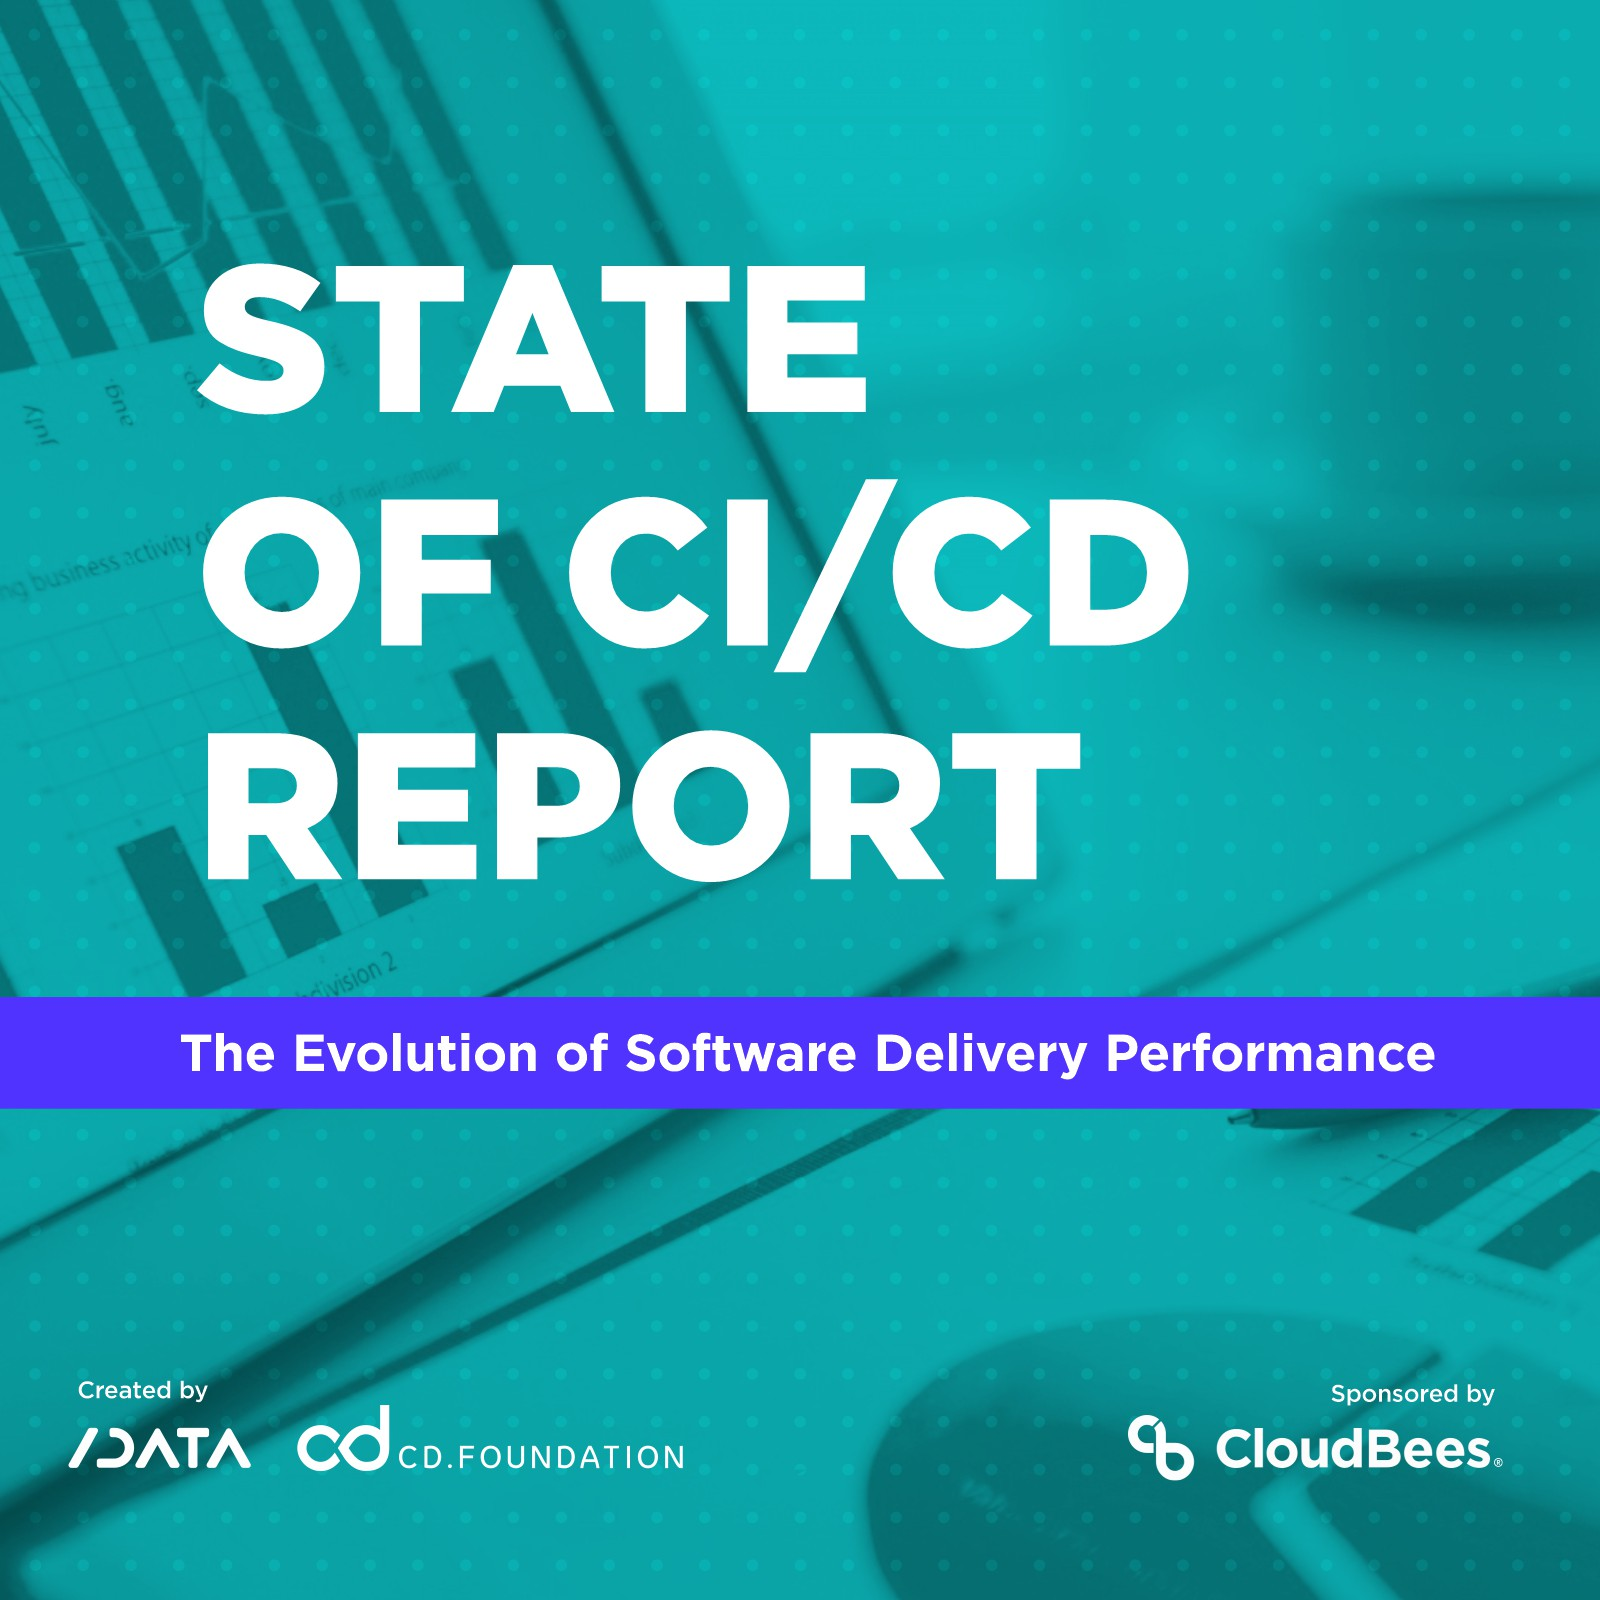
\includegraphics[width=0.4\paperwidth]{img/State of CICD Report square shorthand.jpg}
  \end{textblock*}
  \begin{textblock*}{0.27\paperwidth}(0.60\paperwidth,0.28\paperheight)
    
\includegraphics[width=0.27\paperwidth]{img/state-ci-cd-2024-qr.png}
  \end{textblock*}
\end{blackframe}

\section[CDEvents]{A common specification for Continuous Delivery Events}

\begin{sectionwithpicmediumcentral}[cdeventscon-gradient-16-9.jpg]{
  \begin{textblock*}{0.07\paperwidth}(0.88\paperwidth,0.89\paperheight)
    
\includegraphics[width=0.07\paperwidth]{img/cdf-stacked-color.png}
  \end{textblock*}
}
\end{sectionwithpicmediumcentral}
\note[itemize]{
  \item How many of you are familiar with CDEvents?
}

\begin{grayframe}
  \frametitle{Interoperability}
  \begin{itemize}
    \item Less "Glue Code"
    \item More focus on DevEx \\
          and DevOps metrics
  \end{itemize}
  \begin{textblock*}{0.60\paperwidth}(0.35\paperwidth,0.13\paperheight)
    \includegraphics[width=0.60\paperwidth]{img/cdevents-4-Interoperability.png}
  \end{textblock*}
\end{grayframe}
\note[itemize]{
  \item Various event driven workflows work across tools
  \item SCM Examples
  \item Tekton/Jenkins Example
  \item Argo/Flux Example
  \item Less glue code, more focus on DevEx
}

\begin{textondarkpic}[anthony-yin-okEUu6AMO2Y-unsplash]{%
  Photo by \href{https://unsplash.com/@anthonyin}{\underline{Anthony Yin}}, CC0
  }%
  \frametitle{Evidence Store\\Supply Chain Security}
  \begin{itemize}
    \item Where is this code deployed?\\
          ~~Tracking vulnerabilities\\~
    \item How was this code built?\\
          ~~Audit and compliance\\~
    \item How long did it take?\\
          ~~DevOps Metrics\\~
    \item What's happening right now?\\
          ~~One overview dashboard for all needs
  \end{itemize}
\end{textondarkpic}
\note[itemize]{
  \item Multiple dashboards -> Single point of entry. Backstage example. (Notifications?)
  \item Tracking vulnerabilities
  \item Audit and compliance
  \item Metrics
}

\begin{grayframe}
  \frametitle{IDP and CDEvents}
  \begin{itemize}
    \item Add/swap tools
    \item Consistent Data
    \item Single Dashboard
  \end{itemize}
  ~ \\
  \begin{itemize}
    \item Promotes Collaboration \\
          through Open Source
    \item CDEvents and \href{CNOE.io}{https://cnoe.io}
  \end{itemize}
  \begin{textblock*}{0.60\paperwidth}(0.35\paperwidth,0.13\paperheight)
    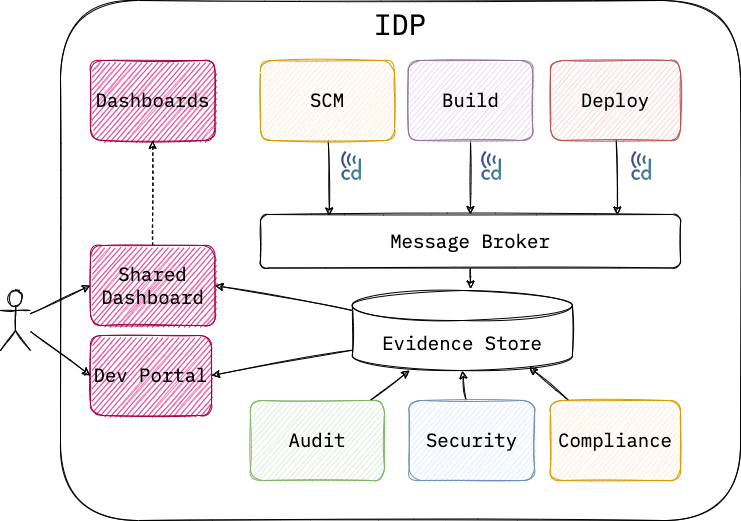
\includegraphics[width=0.60\paperwidth]{img/cdevents-idp-cdevents.png}
  \end{textblock*}
\end{grayframe}
\note[itemize]{
  \item From custom solutions to Open Source
  \item CNOE example, switch and combine tools
}

\begin{grayframe}
  \frametitle{Components}
  \begin{textblock*}{0.80\paperwidth}(0.10\paperwidth,0.15\paperheight)
    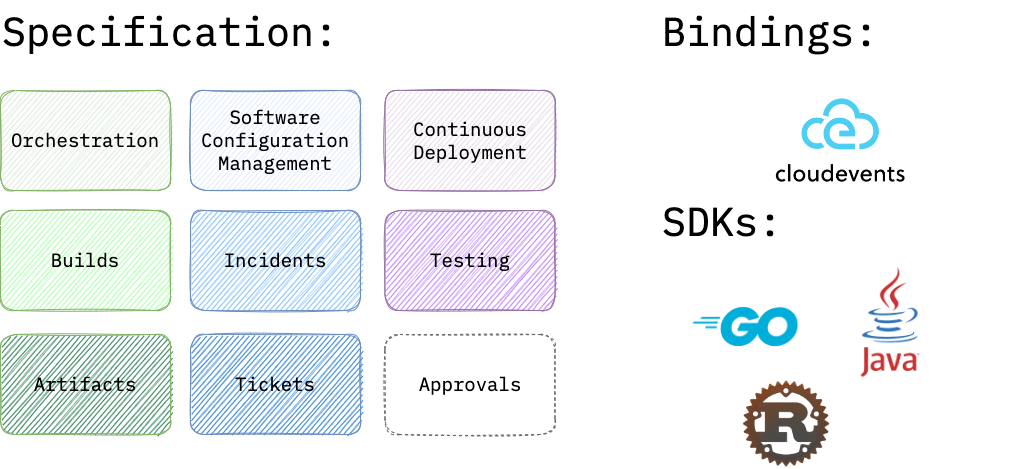
\includegraphics[width=0.80\paperwidth]{img/cdevents-components.png}
  \end{textblock*}
\end{grayframe}
\note[itemize]{
  \item Components slide #14 from google slides
}

\begin{blackframe}
  \frametitle{Community}
  \begin{itemize}
    \item DevOps Engineers\\
            ~~Share your Interoperability pain-points\\~
    \item Tool Maintainer\\
            ~~Adopt CDEvents for your tool\\~
    \item DevOps Vendor\\
            ~~Make it easier for users to integrate\\
            ~~your offering by supporting CDEvents\\~
    \item Love DevOps \& Interoperability\\
            ~~Join us and contribute to CDEvents!
  \end{itemize}
  \begin{textblock*}{0.45\paperwidth}(0.50\paperwidth,0.18\paperheight)
    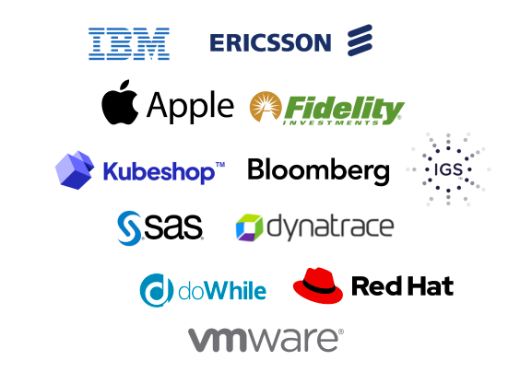
\includegraphics[width=0.45\paperwidth]{img/cdevents-community.png}
  \end{textblock*}
\end{blackframe}
\note[itemize]{
  \item 2. Multiple triggers, 1 dashboard, evidence store (metrics, audit)
  \item Draw two diagrams with IDP
}

\section{Tools Adoption}
\begin{sectionwithpiclargecentral}[clay-banks-LjqARJaJotc-unsplash.jpg]{Photo by \href{https://unsplash.com/@claybanks}{\underline{Clay Banks}}, CC0}
\end{sectionwithpiclargecentral}

\begin{3squares}{Overview}{%
    CDF Projects:
    \begin{itemize}
      \item Jenkins
      \item Spinnaker
      \item Tekton (Experimental)
    \end{itemize}
    ~ \\
    ~ \\
    ~ \\
  }{%
  Other Projects:
  \begin{itemize}
    \item JReleaser
    \item Guah.sh (OpenSSF)
  \end{itemize}
  }{%
  CNCF Projects:
  \begin{itemize}
    \item Testkube
    \item Flux
    \item Argo CD (POC through Notifications)
    \item Harbour (POC)
  \end{itemize}
  ~ \\
  ~ \\
  ~ \\
  Planning:
  \begin{itemize}
    \item Updatecli
    \item Ortelius
    \item Podtato-Head
  \end{itemize}
  }
\end{3squares}
\note[itemize]{
  \item Update the list of tools. updatecli, jreleaser
  \item Add notes for tools
}

\begin{grayframe}
  \frametitle{All Together}
  \begin{textblock*}{0.60\paperwidth}(0.20\paperwidth,0.09\paperheight)
    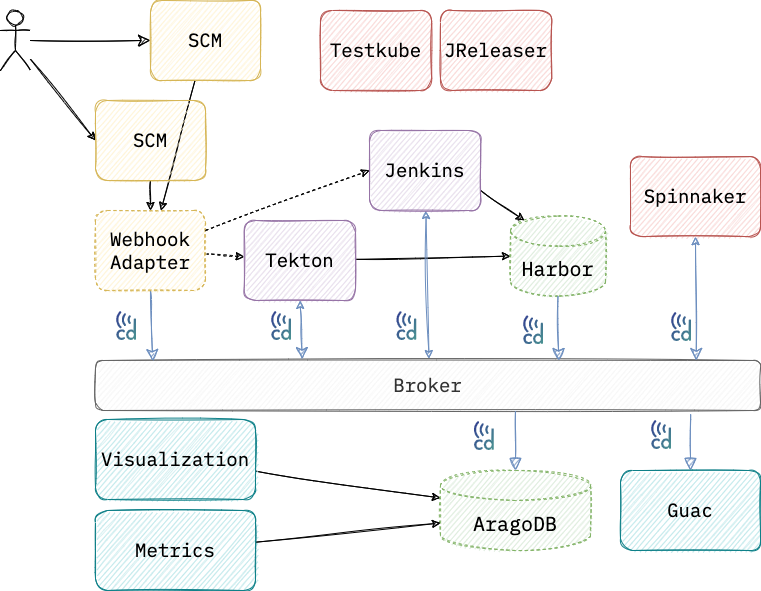
\includegraphics[width=0.60\paperwidth]{img/cdevents-poc.png}
  \end{textblock*}
\end{grayframe}

\begin{3squares}{Successes and challenges}{%
  Challenges:
  \begin{itemize}
    \item Grow the Community
    \item Widespread Adoption
    \item Culture
  \end{itemize}
  ~ \\
  ~ \\
  ~ \\
}{%
Success:
\begin{itemize}
  \item Widespread Interest
  \item Tools Adoption
  \item End Users
\end{itemize}
}{%
Lessons Learnt:
\begin{itemize}
  \item Address specific pain point
  \item Collaborations
\end{itemize}
~ \\
~ \\
~ \\
}
\end{3squares}

\begin{lpicrblack}[nick-fewings-ORSkFfgfEBI-unsplash.jpg]{%
  Photo by \href{https://unsplash.com/@jannerboy62}{\underline{Nick Fewings}}, CC0
  }%
  {%
  \begin{itemize}
    \item OpenTelemetry:\\
          ~~Semantics for Pipeline\\~~Observability
  \end{itemize}
  ~ \\
  \begin{itemize}
    \item \href{CNOE.io}{https://cnoe.io}:\\
          ~~Interoperability layer for IDP
  \end{itemize}
  ~ \\
  \begin{itemize}
    \item Value Stream Management\\
          Interoperability (VSMI) TC
  \end{itemize}
  }%
  {0.35}
  \frametitle{~~~~~~~~~~~~~~~~~~~~~~~~~~~~~~~~~~~~~~~~~~~~~~~~~~~Collaborations}
  \begin{textblock*}{0.15\paperwidth}(0.83\paperwidth,0.25\paperheight)
    \includegraphics[width=0.15\paperwidth]{img/cdevents-Collaborations.png}
  \end{textblock*}
\end{lpicrblack}
\note[itemize]{
  \item Update with google slide #26
}

\section{What's New}
\begin{sectionwithpiclargecentral}[josh-sorenson-MjIMc6uhwrE-unsplash.jpg]{Photo by \href{https://unsplash.com/@joshsorenson}{\underline{Josh Sorenson}}, CC0}
\end{sectionwithpiclargecentral}

\begin{tpicstripedframe}%
  {cdevents-banner-v0-4.png}
  {%
  Linked Events:
  \vspace{0.01\textheight}
  \begin{itemize}
    \item Connect Events
    \item Fast Filtering
    \item Visualization
    \item Audit Trail
  \end{itemize}
  }%
  {%
  Ticket Events:
  \vspace{0.01\textheight}
  \begin{itemize}
    \item Inception to Deployment
    \item E2E Metrics
    \item Ticket Based Automation
    \item Interop.
  \end{itemize}
  }%
  {%
  Custom Events:
  \vspace{0.01\textheight}
  \begin{itemize}
    \item Schema
    \item Custom Types
  \end{itemize}
  \vspace{0.03\textheight}
  Artifact Events:
  \vspace{0.01\textheight}
  \begin{itemize}
    \item SBOM, User
    \item New Predicates
  \end{itemize}
  }%
  {%
  Release Announcement:
  \begin{textblock*}{0.17\paperwidth}(0.78\paperwidth,0.55\paperheight)
    
\includegraphics[width=0.17\paperwidth]{img/cdevents-v4-release-announcement.png}
  \end{textblock*}
  }%
\end{tpicstripedframe}
\note[itemize]{
  \item Update to v0.4 items, various slides
  \item 1. and 2. Content of release
  \item 3. Content of Release, Link to release, link to blog post
}

\section{Roadmap}
\begin{sectionwithpiclargecentral}[dimitar-donovski-yrjB4dYWUZU-unsplash.jpg]{Photo by \href{https://unsplash.com/@dmtrdon}{\underline{Dimitar Donovski}}, CC0}
\end{sectionwithpiclargecentral}

\begin{stripedframe}%
  {%
  CDEvents Roadmap \\
  v0.5 and beyond \\
  ~
  }%
  {%
  Supply Chain Security
  \begin{itemize}
    \item SBOM, Provenance
  \end{itemize}
  \begin{itemize}
    \item Signed Events
  \end{itemize}
  }%
  {%
  New features \\
  ~
  \begin{itemize}
    \item Links, Workflow IDs
    \item Compositions
    \item Releases
  \end{itemize}
  }%
  {%
  Software \& Architecture\\
  ~
  \begin{itemize}
    \item SDKs (JS, Rust)
    \item Adapters
    \item Proof of concept
    \item Broker, Policy
  \end{itemize}
  }%
  {%
  Documentation:
  \begin{itemize}
    \item Reference Architecture
    \item Example events
    \item Example implementations
  \end{itemize}
  }%
\end{stripedframe}
\note[itemize]{
  \item Update Roadmap
  \item Include Experimental CDEvents projects (Visualization, adapter, plugins, more?)
}

\begin{grayframe}
  \frametitle{Conclusions}
  \begin{textblock*}{0.70\paperwidth}(0.15\paperwidth,0.20\paperheight)
    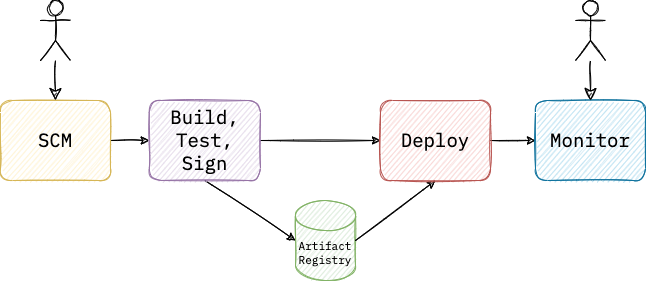
\includegraphics[width=0.70\paperwidth]{img/cdevents-1-no-events.png}
  \end{textblock*}
\end{grayframe}
\note[itemize]{
  \item Google slides #27
}

\section[Thank You]{Thank You!}

\begin{sectionwithpiclargecentral}[carl-jorgensen-5nrnxx_tWe8-unsplash.jpg]{Brecon Beacons, Wales, Photo by \href{https://unsplash.com/@scamartist}{\underline{Carl Jorgensen}}, CC0}
\end{sectionwithpiclargecentral}

\begin{blackframe}
  \frametitle{References}
  \begin{itemize}
    \item \href{https://cdevents.dev}{cdevents.dev, github.com/cdevents}
    \item \href{https://github.com/cdevents/spec/blob/main/CDEvents_Whitepaper.pdf}{github.com/cdevents/spec/blob/main/CDEvents\_Whitepaper.pdf} \\~
    \item \href{https://github.com/jenkinsci/cdevents-plugin}{github.com/jenkinsci/cdevents-plugin}
    \item \href{https://github.com/spinnaker/governance/blob/master/rfc/cdevents-spinnaker.md}{github.com/spinnaker/governance/blob/master/rfc/cdevents-spinnaker.md}
    \item \href{https://github.com/afrittoli/cdeventer}{github.com/afrittoli/cdeventer} \\~
    \item \href{https://github.com/cncf/tag-app-delivery}{github.com/cncf/tag-app-delivery}
    \item \href{https://www.oasis-open.org/committees/tc_home.php?wg_abbrev=vsmi}{VSMI TC @ www.oasis-open.org/committees}
  \end{itemize}
  ~\\
  ~\\
  Andrea Frittoli | \href{mailto:andrea.frittoli@uk.ibm.com}{andrea.frittoli@uk.ibm.com} \\
  \faTwitter ~@blackchip76 | \faGithub ~afrittoli | \faLinkedin ~andreafrittoli
\end{blackframe}
\note[itemize]{
  \item Update references
  \item Blog post v0.4
  \item Slash data report
}

\end{document}
